\documentclass[../main.tex]{subfiles}

\pagestyle{main}
\renewcommand{\chaptermark}[1]{\markboth{\chaptername\ \thechapter}{}}
\setcounter{chapter}{9}

\begin{document}




\chapter{Compactness}\label{sct:10}
\section{Journal}
\begin{definition}\label{dfn:10.1}\marginnote{2/23:}
    We say that a function $f:A\to\R$ is \textbf{bounded} if $f(A)$ is a bounded subset of $\R$. We say that $f$ is \textbf{bounded above} if $f(A)$ is bounded above and that $f$ is \textbf{bounded below} if $f(A)$ is bounded below.\par
    If $f:A\to\R$ is bounded above, we say that $f$ \textbf{attains} (its least upper bound) if there is some $a\in A$ such that $f(a)=\sup f(A)$. Similarly, if $f:A\to\R$ is bounded below, we say that $f$ \textbf{attains} (its greatest lower bound) if there is some $a\in A$ such that $f(a)=\inf f(A)$.
\end{definition}

\begin{exercise}\label{exr:10.2}
    If possible, find examples of each of the following: a picture suffices.
    \begin{enumerate}[label={\alph*)}]
        \item A continuous function on $[1,\infty)$ that is not bounded above.
        \begin{proof}[Example]
            Let $f:[1,\infty)\to\R$ be defined by $f(x)=x$.
            \begin{center}
                \begin{tikzpicture}
                    \footnotesize
                    \draw [->] (-0.4,0) -- (4,0) node[right]{$x$};
                    \draw [->] (0,-0.6) -- (0,3) node[above]{$y$};
                    \draw (1,0.1) -- ++(0,-0.2) node[below]{$1$};

                    \draw [thick,-stealth] (1,1) node[circle,fill,inner sep=1.5pt]{} -- (2.8,2.8);
                \end{tikzpicture}
            \end{center}
        \end{proof}
        \item A continuous function on $[1,\infty)$ that is bounded above but does not attain its least upper bound.
        \begin{proof}[Example]
            Let $f:[1,\infty)\to\R$ be defined by $f(x)=-\frac{1}{x}$.
            \begin{center}
                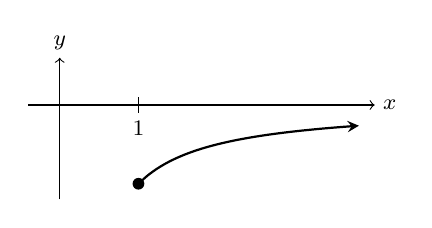
\begin{tikzpicture}
                    \footnotesize
                    \draw [->] (-0.4,0) -- (4,0) node[right]{$x$};
                    \draw [->] (0,-1.2) -- (0,0.6) node[above]{$y$};
                    \draw (1,0.1) -- ++(0,-0.2) node[below]{$1$};

                    \draw [thick,-stealth] plot [domain=1:3.8,smooth] (\x,{-1/\x});
                    \node [circle,fill,inner sep=1.5pt] at (1,-1) {};
                \end{tikzpicture}
            \end{center}
        \end{proof}
        \item A continuous function on $(0,1)$ that is not bounded below.
        \begin{proof}[Example]
            Let $f:(0,1)\to\R$ be defined by $f(x)=-\frac{1}{x}$.
            \begin{center}
                \begin{tikzpicture}
                    \footnotesize
                    \draw [->] (-0.4,0) -- (4,0) node[right]{$x$};
                    \draw [->] (0,-3) -- (0,0.6) node[above]{$y$};
                    \draw (1,0.1) -- ++(0,-0.2) node[below]{$1$};

                    \draw [thick,stealth-] plot [domain=0.36:1,smooth] (\x,{-1/\x}) node[circle,draw,thin,fill=white,inner sep=1.5pt]{};
                \end{tikzpicture}
            \end{center}
        \end{proof}
        \item A continuous function on $(0,1)$ that is bounded below but does not attain its greatest lower bound.
        \begin{proof}[Example]
            Let $f:(0,1)\to\R$ be defined by $f(x)=x$.
            \begin{center}
                \begin{tikzpicture}
                    \footnotesize
                    \draw [->] (-0.4,0) -- (4,0) node[right]{$x$};
                    \draw [->] (0,-0.6) -- (0,3) node[above]{$y$};
                    \draw (1,0.1) -- ++(0,-0.2) node[below]{$1$};

                    \draw [thick] (0,0) node[circle,draw,thin,fill=white,inner sep=1.5pt]{} -- (1,1) node[circle,draw,thin,fill=white,inner sep=1.5pt]{};
                \end{tikzpicture}
            \end{center}
        \end{proof}
    \end{enumerate}
\end{exercise}

\begin{definition}\label{dfn:10.3}
    Let $X$ be a subset of $\R$ and let $\mathcal{G}=\{G_\lambda\}_{\lambda\in\Lambda}$ be a collection of subsets of $\R$. We say that $\mathcal{G}$ is a \textbf{cover} of $X$ if every point of $X$ is in some $G_\lambda$, or in other words:
    \begin{equation*}
        X \subset \bigcup_{\lambda\in\Lambda}G_\lambda
    \end{equation*}
    We say that the collection $\mathcal{G}$ is an \textbf{open cover} if each $G_\lambda$ is open.
\end{definition}

\begin{definition}\label{dfn:10.4}
    Let $X$ be a subset of $\R$. $X$ is \textbf{compact} if for every open cover $\mathcal{G}$ of $X$, there exists a finite subset $\mathcal{G}'\subset\mathcal{G}$ that is also an open cover.
\end{definition}

A good summary of the definition of compactness is "every open cover contains a finite subcover."

\begin{exercise}\label{exr:10.5}
    Show that all finite subsets of $\R$ are compact.
    \begin{proof}
        Let $X$ be an arbitrary finite subset of $\R$. To prove that $X$ is compact, Definition \ref{dfn:10.4} tells us that it will suffice to show that for every open cover $\mathcal{G}$ of $X$, there exists a finite subset $\mathcal{G}'\subset\mathcal{G}$ that is also an open cover. Let $\mathcal{G}$ be an arbitrary open cover of $X$. By Definition \ref{dfn:10.3}, every point $x\in X$ is an element of $G_\lambda$ for some $G_\lambda\in\mathcal{G}$. Thus, for each $x\in X$, let $G_x\in\mathcal{G}$ be a set that contains $x$. Since $X$ is finite, we do not need the axiom of choice to make these selections. Additionally, since there are finitely many $X$, we know that there are finitely many distinct $G_x$\footnote{In fact, the number of $G_x$ is less than or equal to the cardinality of $X$ since we may choose the same $G_x$ for multiple $x$ but may not choose multiple $G_x$ for the same $x$.}. Thus, $\mathcal{G}'=\{G_x\}_{x\in X}$ is finite. Additionally, it is a subset of $\mathcal{G}$ by definition (each $G_x$ is defined to be an element of $\mathcal{G}$). Furthermore, each $G_x$ is open (again, each $G_x$ is an element of $\mathcal{G}$, which is a collection of open sets by definition). Lastly, every point $x\in X$ is an element of $G_x\in\mathcal{G}'$, so $\mathcal{G}'$ is a cover. Therefore, by Definition \ref{dfn:10.3}, $\mathcal{G}'\subset\mathcal{G}$ is a finite open cover of $X$.
    \end{proof}
\end{exercise}

\begin{lemma}\label{lem:10.6}\marginnote{\emph{2/25:}}
    No finite collection of regions covers $\R$.
    \begin{lemma*}
        If $X$ is nonempty, then $\emptyset$ does not cover $X$.
        \begin{proof}
            Suppose for the sake of contradiction that $\emptyset$ covers $X$. By Definition \ref{dfn:1.8}, there exists $x\in X$. It follows by Definition \ref{dfn:10.3} that $x\in\bigcup\emptyset$. But since $\bigcup\emptyset=\emptyset$, we have by Definition \ref{dfn:1.2} that $x\in\emptyset$, contradicting Definition \ref{dfn:1.8}.
        \end{proof}
    \end{lemma*}
    \begin{proof}[Proof of Lemma \ref{lem:10.6}]
        Suppose for the sake of contradiction that $\mathcal{G}$ is a finite collection of regions that covers $\R$. We divide into two cases ($\mathcal{G}=\emptyset$ and $\mathcal{G}\neq\emptyset$). If $\mathcal{G}=\emptyset$, then since $\R$ is nonempty (by Axiom \ref{axm:3.1}), the lemma asserts that $\mathcal{G}$ does not cover $\R$, a contradiction. If $\mathcal{G}\neq\emptyset$, then $\mathcal{G}=\{(a_1,b_1),(a_2,b_2),\dots,(a_n,b_n)\}$. Considering the set $\{a_1,\dots,a_n\}$ of lower bounds of all regions in $\mathcal{G}$, we can determine that it is nonempty and finite since $\mathcal{G}$ itself is nonempty and finite. Thus, by Lemma \ref{lem:3.4}, $\{a_1,\dots,a_n\}$ has a first point $a_i$. It follows by Axiom \ref{axm:3.3} and Definition \ref{dfn:3.3} that there exists a point $x\in\R$ such that $x<a_i$. Since $\mathcal{G}$ is an open cover of $\R$, we know by Definition \ref{dfn:10.3} that $x\in(a_j,b_j)$ for some $(a_j,b_j)\in\mathcal{G}$. But this implies by Equations \ref{eqn:8.1} that $a_j<x$ for some $a_j\in\{a_1,\dots,a_n\}$, contradicting the fact that $x<a_i\leq a_j$ for all $a_j\in\{a_1,\dots,a_n\}$ (the latter inequality being true by Definition \ref{dfn:3.3}).
    \end{proof}
\end{lemma}

\begin{theorem}\label{trm:10.7}
    $\R$ is not compact.
    \begin{proof}
        To prove that $\R$ is not compact, Definition \ref{dfn:10.4} tells us that it will suffice to find an open cover $\mathcal{G}$ of $\R$ such that no finite subset $\mathcal{G}'\subset\mathcal{G}$ exists that is also an open cover. Let $\mathcal{G}$ be the collection of all regions in $\R$.\par
        To confirm that $\mathcal{G}$ is an open cover, Definition \ref{dfn:10.3} tells us that it will suffice to demonstrate that every $x\in\R$ is an element of $R_\lambda$ for some region $R_\lambda\in\mathcal{G}$, and that every $R_\lambda$ is open. For the first condition, let $x$ be an arbitrary element of $\R$. Clearly, we have that $x\in(x-1,x+1)$ where $(x-1,x+1)$ is a region. Thus, $x$ is an element of a set in $\mathcal{G}$, as desired. As to the other condition, we have by Corollary \ref{cly:4.11} that every region (i.e., every set in $\mathcal{G}$) is open, as desired.\par
        To confirm that no finite subset $\mathcal{G}'\subset\mathcal{G}$ exists that is also an open cover, we invoke Lemma \ref{lem:10.6}, which asserts as much. Technically, it forbids $\mathcal{G}'$ from being a cover, but a set that is not a cover cannot be an open cover by Definition \ref{dfn:10.3}.
    \end{proof}
\end{theorem}

\begin{exercise}\label{exr:10.8}
    Show that regions are not compact.
    \begin{proof}
        Let $(a,b)$ be an arbitrary region. To prove that $(a,b)$ is not compact, Definition \ref{dfn:10.4} tells us that it will suffice to find an open cover $\mathcal{G}$ of $\R$ such that no finite subset $\mathcal{G}'\subset\mathcal{G}$ exists that is also an open cover. Let $\mathcal{G}$ be the collection of all regions $(a,c)$ where $c\in(a,b)$.\par
        To confirm that $\mathcal{G}$ is an open cover, Definition \ref{dfn:10.3} tells us that it will suffice to demonstrate that every $x\in(a,b)$ is an element of $(a,c)$ for some $(a,c)\in\mathcal{G}$, and that every $(a,c)$ is open. For the first condition, let $x$ be an arbitrary element of $(a,b)$. Then by Equations \ref{eqn:8.1}, $a<x<b$. It follows by Theorem \ref{trm:5.2} that there exists some $c$ such that $x<c<b$. Since $a<x<c<b$, we have by consecutive applications of Equations \ref{eqn:8.1} that $x\in(a,c)$ and $c\in(a,b)$. The latter result shows that $(a,c)\in\mathcal{G}$, as desired. As to the other condition, we have by Corollary \ref{cly:4.11} that every region (notably including all those in $\mathcal{G}$) is open, as desired.\par
        To confirm that no finite subset $\mathcal{G}'\subset\mathcal{G}$ exists that is also an open cover, let $\mathcal{G}'$ be an arbitrary finite subset of $\mathcal{G}$. We divide into two cases ($\mathcal{G}'=\emptyset$ and $\mathcal{G}'\neq\emptyset$). If $\mathcal{G}'=\emptyset$, then since $(a,b)$ is nonempty, the lemma from Lemma \ref{lem:10.6} asserts that $\mathcal{G}'$ does not cover $(a,b)$, a contradiction. If $\mathcal{G}'\neq\emptyset$, then $\mathcal{G}'=\{(a,c_1),(a,c_2),\dots,(a,c_n)\}$. Considering the set $\{c_1,\dots,c_n\}$ of upper bounds of all regions in $\mathcal{G}'$, we can determine that it is nonempty and finite since $\mathcal{G}'$ itself is nonempty and finite. Thus, by Lemma \ref{lem:3.4}, $\{c_1,\dots,c_n\}$ has a last point $c_i$. Since $c_i\in(a,b)$, Equations \ref{eqn:8.1} assert that $a<c_i<b$. Consequently, by Theorem \ref{trm:5.2}, there exists a point $x\in\R$ such that $c_i<x<b$. Since $a<c_i<x<b$, we have by Equations \ref{eqn:8.1} that $x\in(a,b)$. Since $\mathcal{G}'$ is an open cover of $(a,b)$, we know by Definition \ref{dfn:10.3} that $x\in(a,c_j)$ for some $(a,c_j)\in\mathcal{G}'$. But this implies by Equations \ref{eqn:8.1} that $x<c_j$ for some $c_j\in\{c_1,\dots,c_n\}$, contradicting the fact that $c_j\leq c_i<x$ (the latter inequality being true by Definition \ref{dfn:3.3}).
    \end{proof}
\end{exercise}
\pagebreak

\begin{theorem}\label{trm:10.9}
    If $X$ is compact, then $X$ is bounded.
    \begin{proof}
        We divide into two cases ($X=\emptyset$ and $X\neq\emptyset$). Suppose first that $X=\emptyset$. Then if we let $a,b$ be arbitrary elements of $\R$, it is vacuously true that $a\leq x$ for all $x\in X$ and $x\leq b$ for all $x\in X$. Therefore, by consecutive applications of Definition \ref{dfn:5.6}, $a$ and $b$ are lower and upper bounds of $X$, respectively, and thus $X$ is bounded, as desired.\par
        Now suppose that $X\neq\emptyset$. Let $\mathcal{G}=\{(x-1,x+1)\mid x\in X\}$. To confirm that $\mathcal{G}$ is an open cover of $X$, Definition \ref{dfn:10.3} tells us that it will suffice to demonstrate that every $x\in X$ is an element of some set in $\mathcal{G}$, and that every set in $\mathcal{G}$ is open. For the first condition, let $x$ be an arbitrary element of $X$. Clearly, we have that $x\in(x-1,x+1)$. Additionally, it follows from the fact that $x\in X$ that $(x-1,x+1)\in\mathcal{G}$. Thus, $x$ is an element of a set in $\mathcal{G}$, as desired. As to the other condition, we have by Corollary \ref{cly:4.11} that every region (notably including all those in $\mathcal{G}$) is open, as desired.\par
        Since $\mathcal{G}$ is an open cover of $X$ and $X$ is compact, Definition \ref{dfn:10.4} asserts that there exists a finite subset $\mathcal{G}'$ of $\mathcal{G}$ that is also an open cover of $X$. Since $X$ is nonempty and $\mathcal{G}'$ is a cover of $X$, we have by the lemma from Lemma \ref{lem:10.6} that $\mathcal{G}'\neq\emptyset$. It follows since $\mathcal{G}$ is a collection of regions that $\mathcal{G}'=\{(a_1,b_1),(a_2,b_2),\dots,(a_n,b_n)\}$. Considering the sets $\{a_1,\dots,a_n\}$ of lower bounds of all regions in $\mathcal{G}'$ and $\{b_1,\dots,b_n\}$ of upper bounds of all regions in $\mathcal{G}'$, we can determine that both are nonempty and finite since $\mathcal{G}'$ itself is nonempty and finite. Thus, by consecutive applications of Lemma \ref{lem:3.4}, $\{a_1,\dots,a_n\}$ has a first point $a_i$ and $\{b_1,\dots,b_n\}$ has a last point $b_j$. To confirm that $a_i$ is a lower bound of $X$, Definition \ref{dfn:5.6} tells us that it will suffice to demonstrate that $a_i\leq x$ for all $x\in X$. Let $x$ be an arbitrary element of $X$. Then by Definition \ref{dfn:10.3}, $x\in(a_k,b_k)$ for some $(a_k,b_k)\in\mathcal{G}$. Thus, by Equations \ref{eqn:8.1}, $a_k<x<b_k$. Additionally, since $a_i$ is the first point of $\{a_1,\dots,a_n\}$, Definition \ref{dfn:3.3} asserts that $a_i\leq a_k$. Combining the last two results, we have by transitivity that $a_i<x$, which we may weaken to $a_i\leq x$, as desired. The proof that $b_j$ is an upper bound is symmetric. Therefore, since $X$ has a lower and an upper bound, Definition \ref{dfn:5.6} implies that $X$ is bounded.
    \end{proof}
\end{theorem}

\begin{lemma}\label{lem:10.10}
    Let $X\subset\R$ and $p\in\R\setminus X$. Then $\mathcal{G}=\{\ext(a,b)\mid p\in(a,b)\}$ is an open cover of $X$.
    \begin{proof}
        To prove that $\mathcal{G}$ is an open cover of $X$, Definition \ref{dfn:10.3} tells us that it will suffice to show that every $x\in X$ is an element of some set in $\mathcal{G}$, and that every set in $\mathcal{G}$ is open. For the first condition, let $x,p$ be arbitrary elements of $X,\R\setminus X$, respectively. Since $x,p$ are elements of disjoint sets by Script \ref{sct:1}, we know that $x\neq p$. Thus, we can apply Theorem \ref{trm:3.22} to learn that there exist disjoint regions $(c,d)$ and $(a,b)$ containing $x$ and $p$, respectively. We now seek to verify that $x\in\ext(a,b)$. To do so, Definition \ref{dfn:3.15} tells that it will suffice to verify that $x\notin(a,b)$, $x\neq a$, and $x\neq b$. First, suppose for the sake of contradiction that $x\in(a,b)$. Then since $x\in(c,d)$, too, $x\in(a,b)\cap(c,d)$, contradicting Definition \ref{dfn:1.9} and the fact that $(a,b),(c,d)$ are disjoint. Second, suppose for the sake of contradiction that $x=a$. Since $x\in(c,d)$, we have by Equations \ref{eqn:8.1} that $c<x=a<d$. We divide into two cases ($d\leq b$ and $b<d$). If $d\leq b$, then by Theorem \ref{trm:5.2}, we can choose $z$ such that $c<x=a<z<d\leq b$. It follows by the same logic as in the first case that $z\in(a,b)\cap(c,d)$, and we arrive at the same contradiction. If $b<d$, then we similarly choose $c<x=a<z<b<d$, and arrive at the same contradiction again. The proof of the third claim is symmetric to that of the second. Therefore, $x\in\ext(a,b)$, so we have by the definition of $\mathcal{G}$ that $x$ is an element of a set in $\mathcal{G}$, as desired. As to the other condition, we have by Corollary \ref{cly:4.21} that every exterior of a region (notably including all those in $\mathcal{G}$) is open, as desired.
    \end{proof}
\end{lemma}

\begin{theorem}\label{trm:10.11}
    If $X$ is compact, then $X$ is closed.
    \begin{proof}
        We divide into two cases ($X=\emptyset$ and $X\neq\emptyset$). Suppose first that $X=\emptyset$. Then by Theorem \ref{trm:4.2}, $X$ is closed, as desired.\par
        Now suppose that $X\neq\emptyset$, and suppose for the sake of contradiction that $X$ is not closed. Then by Definition \ref{dfn:4.1}, there exists a limit point $p$ of $X$ such that $p\notin X$. Since $p\in\R$ and $p\notin X$, Definition \ref{dfn:1.11} implies that $p\in\R\setminus X$. Thus, by Lemma \ref{lem:10.10}, $\mathcal{G}=\{\ext(a,b)\mid p\in(a,b)\}$ is an open cover of $X$. Additionally, since $X$ is compact by hypothesis, we have by Definition \ref{dfn:10.4} that there exists a finite subset $\mathcal{G}'\subset\mathcal{G}$ that is also an open cover of $X$. Since $X$ is nonempty and $\mathcal{G}'$ is as cover of $X$, we have by the lemma from Lemma \ref{lem:10.6} that $\mathcal{G}'\neq\emptyset$. It follows since $\mathcal{G}$ is a collection of exteriors of regions that $\mathcal{G}'=\{\ext(a_1,b_1),\ext(a_2,b_2),\dots,\ext(a_n,b_n)\}$. Considering the sets $\{a_1,\dots,a_n\}$ and $\{b_1,\dots,b_n\}$, we can determine that both are nonempty and finite since $\mathcal{G}'$ itself is nonempty and finite. Thus, by consecutive applications of Lemma \ref{lem:3.4}, $\{a_1,\dots,a_n\}$ has a last point $a_i$ and $\{b_1,\dots,b_n\}$ has a first point $b_j$. We now seek to verify that $p\in(a_i,b_j)$. By consecutive applications of the definition of $\mathcal{G}$, $p\in(a_i,b_i)$ and $p\in(a_j,b_j)$. Consequently, by consecutive applications of Equations \ref{eqn:8.1}, $a_i<p<b_i$ and $a_j<p<b_j$. Since $a_i<p<b_j$, we have by Equations \ref{eqn:8.1} that $p\in(a_i,b_j)$, as desired. Thus, since $p\in(a_i,b_j)$ and $p\in LP(X)$, Definition \ref{dfn:3.13} asserts that $(a_i,b_j)\cap(X\setminus\{p\})\neq\emptyset$. Consequently, by Definition \ref{dfn:1.8}, there exists some $x\in(a_i,b_j)\cap(X\setminus\{p\})$. Thus, by Definitions \ref{dfn:1.6} and \ref{dfn:1.11}, $x\in(a_i,b_j)$ and $x\in X$. Since $\mathcal{G}'$ is an open cover of $X$, it follows from the latter condition by Definition \ref{dfn:10.3} that $x\in\ext(a_k,b_k)$ for some $\ext(a_k,b_k)\in\mathcal{G}'$. Consequently, by Lemma \ref{lem:3.16}, $x<a_k$ or $b_k<x$. We now divide into two cases. If $x<a_k$, this contradicts the fact that $a_k\leq a_i<x$ (the former inequality being true by Definition \ref{dfn:3.3} since $a_i$ is the last point of $\{a_1,\dots,a_n\}$). If $b_k<x$, we arrive at a symmetric contradiction.
    \end{proof}
\end{theorem}

It will turn out that the two properties of compactness in Theorems \ref{trm:10.9} and \ref{trm:10.11} characterize compact sets completely, meaning that every bounded closed set is compact. We will see this in Theorem \ref{trm:10.16}. First, however, we need some preliminary results.\par
For the next three statements, fix points $a,b\in\R$ and suppose $\mathcal{G}$ is an open cover of $[a,b]$.

\begin{lemma}\label{lem:10.12}
    For all $s\in[a,b]$, there exists $G\in\mathcal{G}$ and $p,q\in\R$ such that $p<s<q$ and $[p,q]\subset G$.
    \begin{proof}
        Let $s$ be an arbitrary element of $[a,b]$. Since $\mathcal{G}$ is an open cover of $[a,b]$, Definition \ref{dfn:10.3} implies that there exists a $G\in\mathcal{G}$ such that $s\in G$ and $G$ is open. It follows from the latter condition by Theorem \ref{trm:4.10} that there exists a region $(x,y)$ such that $s\in(x,y)$ and $(x,y)\subset G$. Since $s\in(x,y)$, we have by Equations \ref{eqn:8.1} that $x<s<y$. Thus, by consecutive applications of Theorem \ref{trm:5.2}, we can pick $p,q\in\R$ such that $x<p<s<q<y$. Clearly, $p<s<q$. To verify that $[p,q]\subset G$, Definition \ref{dfn:1.3} tells us that it will suffice to confirm that every $z\in[p,q]$ is an element of $G$. Let $z$ be an arbitrary element of $[p,q]$. Then by Equations \ref{eqn:8.1}, $p\leq z\leq q$. It follows since $x<p<q<y$ that $x<p\leq z\leq q<y$, meaning by Equations \ref{eqn:8.1} that $z\in(x,y)$. Since $(x,y)\subset G$ by definition, we have by Definition \ref{dfn:1.3} that $z\in G$, as desired.
    \end{proof}
\end{lemma}

\begin{lemma}\label{lem:10.13}\marginnote{\emph{3/2:}}
    Let $X$ be the set of all $x\in\R$ that are \textbf{reachable} from $a$, by which we mean the following: there exist $n\in\N\cup\{0\}$, $x_0,...,x_n\in\R$, and $G_1,\dots,G_n\in\mathcal{G}$ such that $a=x_0<x_1<\cdots<x_{n-1}<x_n=x$ and $[x_{i-1},x_i]\subset G_i$ for $i=1,\dots,n$. Note in particular that $a\in X$, by choosing $n=0$. Then the point $b$ is not an upper bound for $X$.
    \begin{proof}
        Suppose for the sake of contradiction that $b$ is an upper bound of $X$. We know by hypothesis that $a\in X$. Thus, $X$ is a nonempty set that is bounded above, so by Theorem \ref{trm:5.17}, $\sup X$ exists. Let $s=\sup X$. Since $b$ is an upper bound of $X$, we have by Definition \ref{dfn:5.7} that $s\leq b$. Additionally, since $a\in X$, we have by Definitions \ref{dfn:5.7} and \ref{dfn:5.6} that $a\leq s$. Combining these last two results, we have by Equations \ref{eqn:8.1} that $s\in[a,b]$. Thus, by Lemma \ref{lem:10.12}, there exists $G\in\mathcal{G}$ and $p,q\in\R$ such that $p<s<q$ and $[p,q]\subset G$. Additionally, we have by Lemma \ref{lem:5.11} that there exists an $x\in X$ such that $p<x\leq s$. Since $p<x\leq s<q$, we have by Equations \ref{eqn:8.1} that $x\in[p,q]$. It follows by Definition \ref{dfn:1.3} since $[p,q]\subset G$ that $x\in G$. Furthermore, by Theorem \ref{trm:5.2}, there exists $s'\in\R$ such that $s<s'<q$. We will now demonstrate that $s'\in X$, which will contradict the previously proven statement that $s$ is an upper bound on $X$.\par
        To demonstrate that $s'\in X$, the definition of $X$ tells us that it will suffice to confirm that there exist $n+1\in\N\cup\{0\}$, $x_0,\dots,x_{n+1}\in\R$, and $G_1,\dots,G_{n+1}\in\mathcal{G}$ such that $a=x_0<\cdots<x_{n+1}=s'$ and $[x_{i-1},x_i]\subset G_i$ for $i=1,\dots,n+1$. To begin, since $x\in X$, we have that there exist $n\in\N\cup\{0\}$, $x_0,\dots,x_n\in\R$, and $G_1,\dots,G_n\in\mathcal{G}$ such that $a=x_0<\cdots<x_n=x$ and $[x_{i-1},x_i]\subset G_i$ for $i=1,\dots,n$. Let $x_{n+1}=s'$ and $G_{n+1}=G$. Then since we can carry over all of the variable assignments from the definition of $x$ and add in $x_n=x\leq s<s'=x_{n+1}$ as well as $[x_n,x_{n+1}]=[x,s']\subset[p,q]\subset G=G_{n+1}$, we have that $s'\in X$, as desired.
    \end{proof}
\end{lemma}

\begin{theorem}\label{trm:10.14}
    The set $[a,b]$ is compact.
    \begin{proof}
        To prove that $[a,b]$ is compact, Definition \ref{dfn:10.4} tells us that it will suffice to show that for every open cover $\mathcal{G}$ of $[a,b]$, there exists a finite subset $\mathcal{G}'\subset\mathcal{G}$ that is also an open cover. Let $\mathcal{G}$ be an arbitrary open cover of $[a,b]$. By Lemma \ref{lem:10.13}, $b$ is not an upper bound of $X$ where $X$ is the set of all $x\in\R$ that are reachable from $a$. Thus, by Definition \ref{dfn:5.6}, there exists an $x\in X$ such that $x>b$. Since $x\in X$, we have by Lemma \ref{lem:10.13} that there exist $n\in\N\cup\{0\}$, $x_0,\dots,x_n\in\R$, and $G_1,\dots,G_n\in\mathcal{G}$ such that $a=x_0<\cdots<x_n=x$ and $[x_{i-1},x_i]\subset G_i$ for $i=1,\dots,n$. Let $\mathcal{G}'=\{G_1,\dots,G_n\}$. We will now show that $\mathcal{G}'$ is finite, a subset of $\mathcal{G}$, and an open cover of $[a,b]$.\par
        Clearly, $\mathcal{G}'$ is finite.\par
        Since every element of $\mathcal{G}'$ is an element of $\mathcal{G}$ by definition, we have by Definition \ref{dfn:1.3} that $\mathcal{G}'\subset\mathcal{G}$.\par
        To show that $\mathcal{G}'$ is an open cover of $[a,b]$, Definition \ref{dfn:10.3} tells us that it will suffice to verify that every $y\in[a,b]$ is an element of $G_i$ for some $G_i\in\mathcal{G}'$, and that every $G_i$ is open. For the first condition, suppose for the  sake of contradiction that there exists a $y\in[a,b]$ such that $y\notin G_i$ for any $G_i\in\mathcal{G}'$. Then since $[x_{i-1},x_i]\subset G_i$ for all $i=1,\dots,n$, $y\notin[x_{i-1},x_i]$ for any $i=1,\dots,n$. It follows from Equations \ref{eqn:8.1} that $y<x_{i-1}$ or $y>x_i$ for all $i=1,\dots,n$. In particular, we have that $y<x_0=a$ or $y>x_n=x$. We now divide into two cases. If $y<a$, then by Equations \ref{eqn:8.1}, $y\notin[a,b]$, a contradiction. If $y>x$, then since $x>b$, we have that $y>b$, which implies by Equations \ref{eqn:8.1} that $y\notin[a,b]$, a contradiction. As to the other condition, we have by the definition of $\mathcal{G}$ that every $G_i$ is open, as desired.
    \end{proof}
\end{theorem}

\begin{theorem}\label{trm:10.15}
    A closed subset $Y$ of a compact set $X\subset\R$ is compact.
    \begin{lemma*}
        $Y$ is closed in $X$ if and only if $Y$ is closed.
        \begin{proof}
            Suppose first that $Y$ is closed in $X$. Then by Definition \ref{dfn:8.11}, $Y=X\cap B$ where $B$ is closed. Additionally, since $X$ is compact, Theorem \ref{trm:10.11} asserts that $X$ is closed. Therefore, since $Y$ is the intersection of two closed sets, we have by Theorem \ref{trm:4.16} that $Y$ is closed, as desired.\par
            Now suppose that $Y$ is closed. Since $Y=X\cap Y$ by Script \ref{sct:1}, we have by Definition \ref{dfn:8.11} that $Y$ is closed in $X$, as desired.
        \end{proof}
    \end{lemma*}
    \begin{proof}[Proof of Theorem \ref{trm:10.15}]
        To prove that $Y$ is compact, Definition \ref{dfn:10.4} tells us that it will suffice to show that for every open cover $\mathcal{G}$ of $Y$, there exists a finite subset $\mathcal{G}'\subset\mathcal{G}$ that is also an open cover. To do this, we will first demonstrate that $\mathcal{H}=\mathcal{G}\cup\{\R\setminus Y\}$ is an open cover of $X$. It will follow that there exists a finite subset $\mathcal{H}'\subset\mathcal{H}$ that is an open cover of $X$. Lastly, we will demonstrate that $\mathcal{G}'=\mathcal{H}'\setminus\{\R\setminus Y\}$ is the desired finite open cover subset of $\mathcal{G}$.\par\smallskip
        Let $\mathcal{G}$ be an arbitrary open cover of $Y$, and let $\mathcal{H}=\mathcal{G}\cup\{\R\setminus Y\}$. To demonstrate that $\mathcal{H}$ is an open cover of $X$, Definition \ref{dfn:10.3} tells us that it will suffice to confirm that every $x\in X$ is an element of $H$ for some $H\in\mathcal{H}$, and that every $H$ is open. For the first condition, let $x$ be an arbitrary element of $X$. We divide into two cases ($x\in Y$ and $x\notin Y$). If $x\in Y$, then since $\mathcal{G}$ is an open cover of $Y$, Definition \ref{dfn:10.3} implies that $x\in G$ for some $G\in\mathcal{G}$. But since $\mathcal{G}\subset\mathcal{H}$, $x\in G$ for some $G\in\mathcal{H}$, as desired. On the other hand, if $x\notin Y$, then this combined with the fact that $x\in\R$ implies by Definition \ref{dfn:1.11} that $x\in\R\setminus Y\in\mathcal{H}$, as desired. As to the other condition, let $H$ be an arbitrary element of $\mathcal{H}$. We divide into two cases ($H\in\mathcal{G}$ and $H\notin\mathcal{G}$). If $H\in\mathcal{G}$, then by Definition \ref{dfn:10.3}, $H$ is open, as desired. On the other hand, if $H\notin\mathcal{G}$, then $H=\R\setminus Y$ by Script \ref{sct:1}. It follows since $Y$ is closed by Definition \ref{dfn:4.8} that $\R\setminus Y$ is open, so $H$ is open, as desired.\par
        Since $\mathcal{H}$ is an open cover of $X$ and $X$ is compact, we have by Definition \ref{dfn:10.4} that there exists a finite subset $\mathcal{H}'\subset\mathcal{H}$ that is also an open cover of $X$. Let $\mathcal{G}'=\mathcal{H}'\setminus\{\R\setminus Y\}$. By Script \ref{sct:1}, $\mathcal{G}'\subset\mathcal{G}$. Additionally, since $\mathcal{H}'$ is finite, Script \ref{sct:1} also implies that $\mathcal{G}'$ is finite. However, to demonstrate that $\mathcal{G}'$ is an open cover of $Y$, Definition \ref{dfn:10.3} tells us that we must confirm that every $y\in Y$ is an element of $G$ for some $G\in\mathcal{G}'$, and that every $G$ is open. For the first condition, let $y$ be an arbitrary element of $Y$. Then since $Y\subset X$, Definition \ref{dfn:10.3} asserts that $y\in H$ for some $H\in\mathcal{H}'$. Additionally, since $y\in Y$, Definition \ref{dfn:1.11} implies that $y\notin\R\setminus Y$. Thus, $H\neq\R\setminus Y$, which implies by Definition \ref{dfn:1.11} that $H\in\mathcal{H}'\setminus\{\R\setminus Y\}=\mathcal{G}'$. Therefore, $y\in H$ for some $H\in\mathcal{G}'$, as desired. As to the other condition, since every $G\in\mathcal{G}'$ is an element of $\mathcal{G}$ (i.e., open by Definition \ref{dfn:10.3}), every $G\in\mathcal{G}'$ is open, as desired.
    \end{proof}
\end{theorem}

\begin{theorem}\label{trm:10.16}
    Let $X\subset\R$. $X$ is compact if and only if $X$ is closed and bounded.
    \begin{proof}
        Suppose first that $X$ is compact. Then by Theorems \ref{trm:10.11} and \ref{trm:10.9}, respectively, $X$ is closed and bounded.\par
        Now suppose that $X$ is closed and bounded. It follows from the latter condition by Definition \ref{dfn:5.6} that $X$ has a lower bound $a$ and an upper bound $b$. Constructing the region $[a,b]$, we have from Theorem \ref{trm:10.14} that $[a,b]$ is compact. Additionally, we know that $X\subset[a,b]$ since $x\in X$ implies by consecutive applications of Definition \ref{dfn:5.6} that $a\leq x\leq b$, from which it follows by Equations \ref{eqn:8.1} that $x\in[a,b]$. Thus, $X$ is a closed (by hypothesis) subset of a compact set, so by Theorem \ref{trm:10.15}, $X$ is compact.
    \end{proof}
\end{theorem}

\begin{lemma}\label{lem:10.17}
    A compact set $X\subset\R$ with no limit points must be finite.
    \begin{proof}
        Suppose for the sake of contradiction that $X$ is infinite, and let $x$ be an arbitrary element of $X$. Since $X$ has no limit points, we know that $x\notin LP(X)$. Thus, by Definition \ref{dfn:3.13}, there exists a region $R_x$ with $x\in R_x$ such that $R_x\cap(X\setminus\{x\})=\emptyset$. Let $\mathcal{G}=\bigcup_{x\in X}R_x$, where $R_x$ is similarly defined for each $x\in X$. Then since every $x\in R_x\in\mathcal{G}$ and every $R_x$ is open by Corollary \ref{cly:4.11}, Definition \ref{dfn:10.3} implies that $\mathcal{G}$ is an open cover of $X$. It follows since $X$ is compact that there exists a finite subset of $\mathcal{G}'\subset\mathcal{G}$ that is also an open cover of $X$. Additionally, since $\mathcal{G}'$ is finite whereas $\mathcal{G}$ is infinite (infinitely many $x$ imply infinitely many $R_x$ since each $R_x$ contains only one $x$), we know that $\mathcal{G}'\neq\mathcal{G}$. Thus, there exists an $R_x\in\mathcal{G}$ such that $R_x\notin\mathcal{G}'$. However, since $\mathcal{G}'$ is an open cover of $X$, Definition \ref{dfn:10.3} implies that $x\in R_y$ for some $R_y\in\mathcal{G}'$ where $y\neq x$. But since $x\in R_y$, $x\in X$, and $x\neq y$, it follows by Script \ref{sct:1} that $R_y\cap(X\setminus\{y\})\neq\emptyset$, a contradiction.
    \end{proof}
\end{lemma}

\begin{theorem}\label{trm:10.18}
    Every bounded infinite subset of $\R$ has at least one limit point.
    \begin{proof}
        Suppose for the sake of contradiction that $X$ is a bounded, infinite subset of $\R$ with no limit points. Since $X$ has no limit points, it is vacuously true that it contains all of its limit points. Thus, by Definition \ref{dfn:4.1}, $X$ is closed. This combined with the fact that $X$ is bounded implies by Theorem \ref{trm:10.16} that $X$ is compact. But this combined with the fact that $X$ has no limit points implies by Lemma \ref{lem:10.17} that $X$ is finite, a contradiction.
    \end{proof}
\end{theorem}




\end{document}